%------------------------------------------------------------------------------
% Author(s):
% Varaun Ramgoolie
% Copyright:
%  Copyright (C) 2020 Brad Bachu, Arjun Mohammed, Varaun Ramgoolie, Nicholas Sammy
%
%  This file is part of Applied-Mathematics-Unit2 and is distributed under the
%  terms of the MIT License. See the LICENSE file for details.
%
%  Description:
%     Linear Programming graph for 2012 q1
%------------------------------------------------------------------------------

\documentclass[crop,tikz]{standalone}
\usepackage{pgfplots}
\usepackage{../../../../src/tikzappmath}
\usetikzlibrary{patterns}

\begin{document}
	
	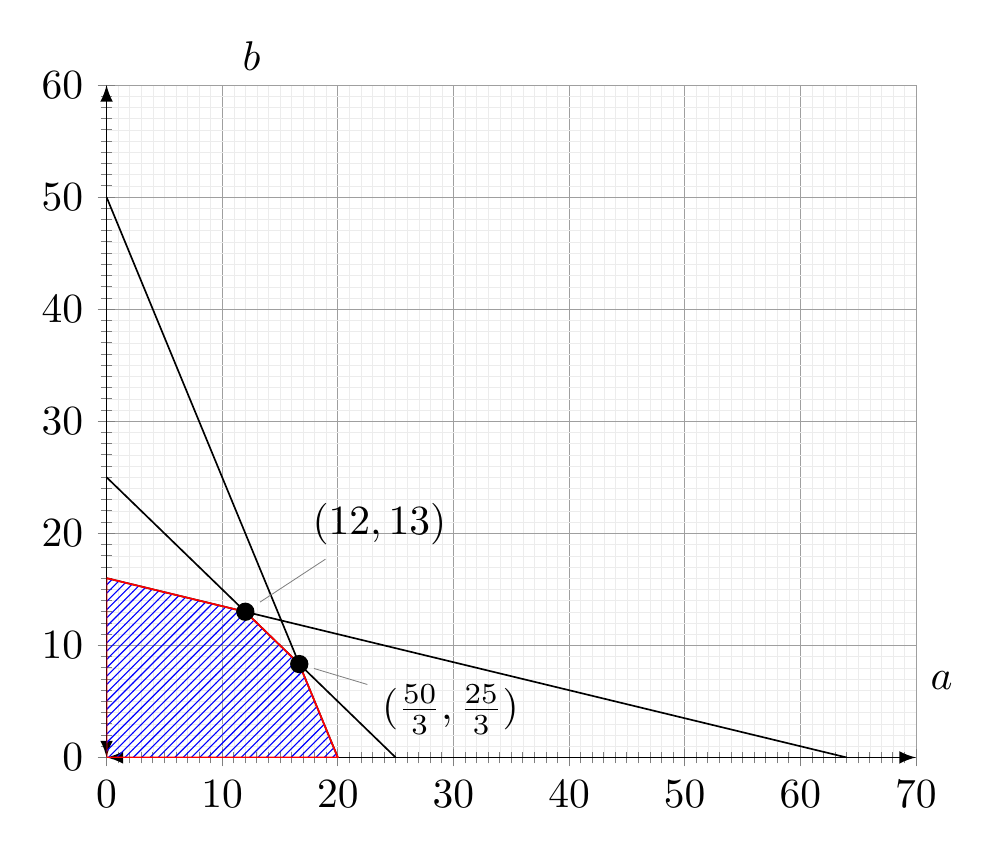
\begin{tikzpicture}[scale=1.5]
	\begin{axis}
		[
		xmin=-0,xmax=70,
		ymin=0,ymax=60,
		grid=both,
		grid style={line width=.1pt, draw=darkgray!10},
		major grid style={line width=.2pt,draw=darkgray!50},
		axis lines=left,
		minor tick num=9,
		enlargelimits={abs=0},
		axis line style={latex-latex},
		samples=100,
		domain = -20:20,
		ytick={0,10,...,60},
		xlabel={$a$},
		ylabel={$b$},
		x label style={at={(axis description cs:1,0.15)},anchor=north west},
		y label style={at={(axis description cs:0.15,1)},anchor=south west, rotate=-90}
		]
		
		\addplot [mark=dot] coordinates{(25,0)  (0,25)};
		
		\addplot [mark=dot] coordinates {(64,0) (0,16)};
		
		\addplot [mark=dot] coordinates {(20,0) (0,50)};
		
		\addplot [red,pattern=north east lines,pattern color=blue] coordinates {(0,16) (12,13) (50/3, 25/3) (20,0)} \closedcycle;	
		
		\addplot [mark=*] coordinates{(12,13)};
		
		\node [pin=355:{$(\frac{50}{3},\frac{25}{3})$}] at (axis cs:50/3, 25/3) {};
		
		\addplot [mark=*] coordinates{(50/3, 25/3)};
		
		\node [pin=45:{$(12,13)$}] at (axis cs:12,13) {};
		
		\end{axis}
	\end{tikzpicture}
	
\end{document}